The major sources of background events are summarized in Section~\ref{ssww13tev:background_overview}, and the methods used to estimate them are detailed in this section.  
Prompt backgrounds from $ZZ$ and $t\bar{t}V$ are estimated directly from MC simulations.
The shape of the $WZ$ and $V\gamma$ backgrounds are taken from MC, and the predicted yeilds are normalized to the data predictions in dedicated control regions, as outlined in Sections~\ref{ssww13tev:wz} and \ref{ssww13tev:wgamma}, respectively.
Opposite sign events with a charge misidentified electron are estimated by a data-driven background method which is summarized in Section~\ref{ssww13tev:charge_misid}.
Finally, a \emph{fake factor} method is used to estimate the contributions from non-prompt backgrounds and is the subject of Section~\ref{ssww13tev:fake_factor}.

\subsection{Estimation of the $WZ$ background}\label{ssww13tev:wz}
The dominant background involving prompt leptons comes from $WZ$+jets events.
The contribution is estimated from MC simulation and normalized to data in a control region enriched in $WZ$ events defined by the same event selection as Table~\ref{tab:ssww13tev_event_selection} for the signal region, with the following changes applied to increase the purity of the $WZ$ process:
\begin{itemize}
\item The third lepton veto is inverted, requiring a third lepton with $\pt > 15\gev$
\item Two of the leptons must make a same-flavor opposite-sign pair. If more than one pair exists, the one with $m_{ll}$ closest to the $Z$ boson mass is chosen.
\item The trilepton invariant mass is required to be $m_{lll} > 106\gev$ to reduce contributions from $Z\gamma$ and $Z$+jets
\end{itemize}

Once the event yields in the control region are calculated, they are propagated to the final signal region fit, detailed in Section~\ref{ssww13tev:xsec} \TODO{update reference with proper subsection once it's written}, in a single bin combining all the lepton channels.
The systematic uncertainties of the $WZ$ background are also calculated at this time.
The event yields for the $WZ$ control region are listed in Table~\ref{tab:ssww13tev_wzcr_yields}, and distributions of the leading lepton $\pt$ and $\eta$ as well as trilepton invariant mass $m_{lll}$ are found in Figures~\ref{fig:ssww13tev_wzcr_lep0} and \ref{fig:ssww13tev_wzcr_mlll}, respectively.

\begin{table}[htbp]
  \centering
  \begin{tabular}{l r}
    \multicolumn{2}{c}{Event yields in the $WZ$ control region} \\
    \hline\hline
    $WZ$     & $197.9\pm 1.4$ \\
    $ZZ$     & $14.1\pm 0.3$ \\
    Triboson & $1.26\pm 0.1$ \\
    top      & $10.8\pm 1.1$ \\
    $Z\gamma$& $3.1\pm 1.1$ \\
    $Z$+jets & $2.5\pm 1.4$ \\
    \hline
    Total prediction & $229.7\pm 2.5$ \\
    Data             & $201 \pm 14.2$ \\
    \hline
  \end{tabular}
  \caption{Event yields in the $WZ$ control region before normalization.  All lepton flavor channels are combined.}
  \label{tab:ssww13tev_wzcr_yields}
\end{table}

\begin{figure}[htbp]
  \centering
  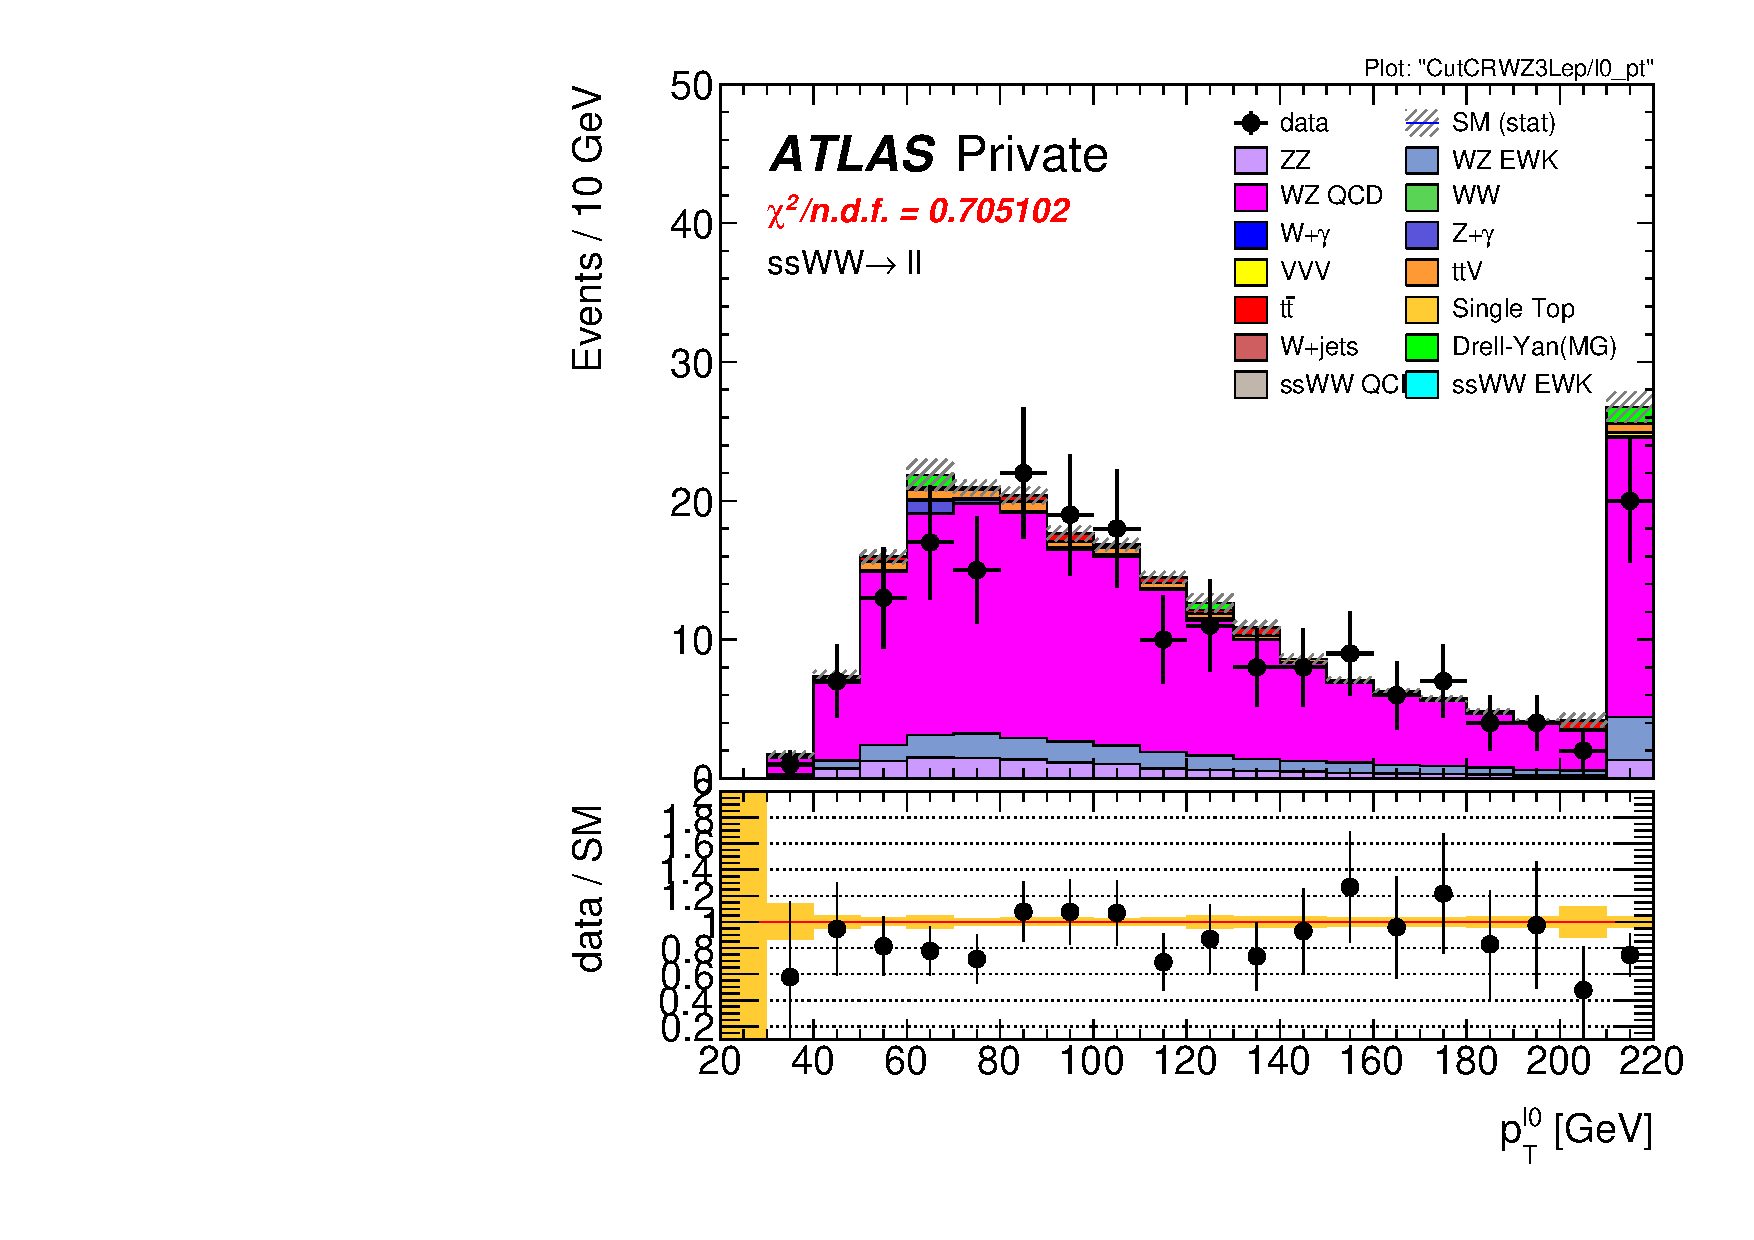
\includegraphics[width=.48\textwidth]{figs/ssww_13tev/backgrounds/wz/ll-CutCRWZ3Lep-l0_pt-lin}
  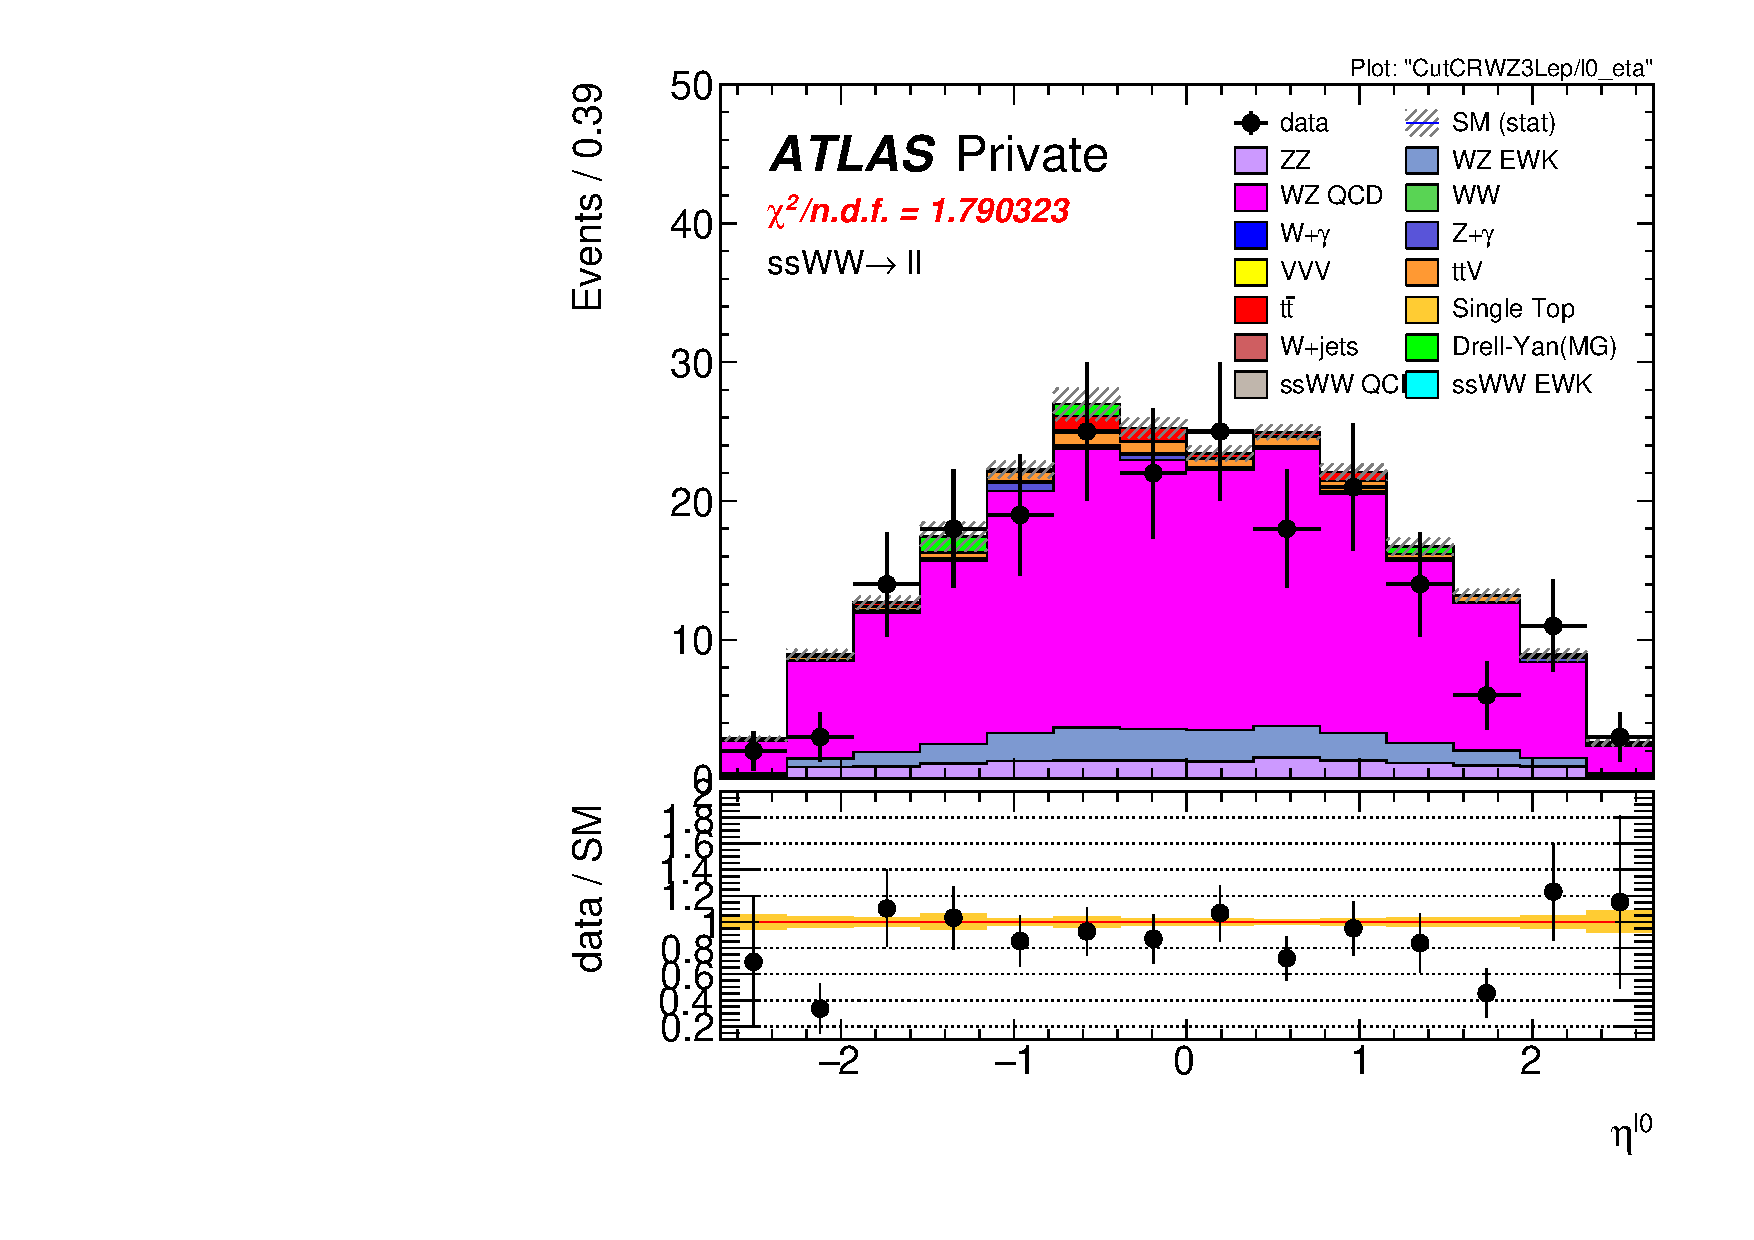
\includegraphics[width=.48\textwidth]{figs/ssww_13tev/backgrounds/wz/ll-CutCRWZ3Lep-l0_eta-lin}
  \caption{Leading lepton $\pt$ (left) and $\eta$ (right) distributions in the $WZ$ control region before normalization.  All lepton channels are combined.}
  \label{fig:ssww13tev_wzcr_mlll}
\end{figure}

\begin{figure}[htbp]
  \centering
  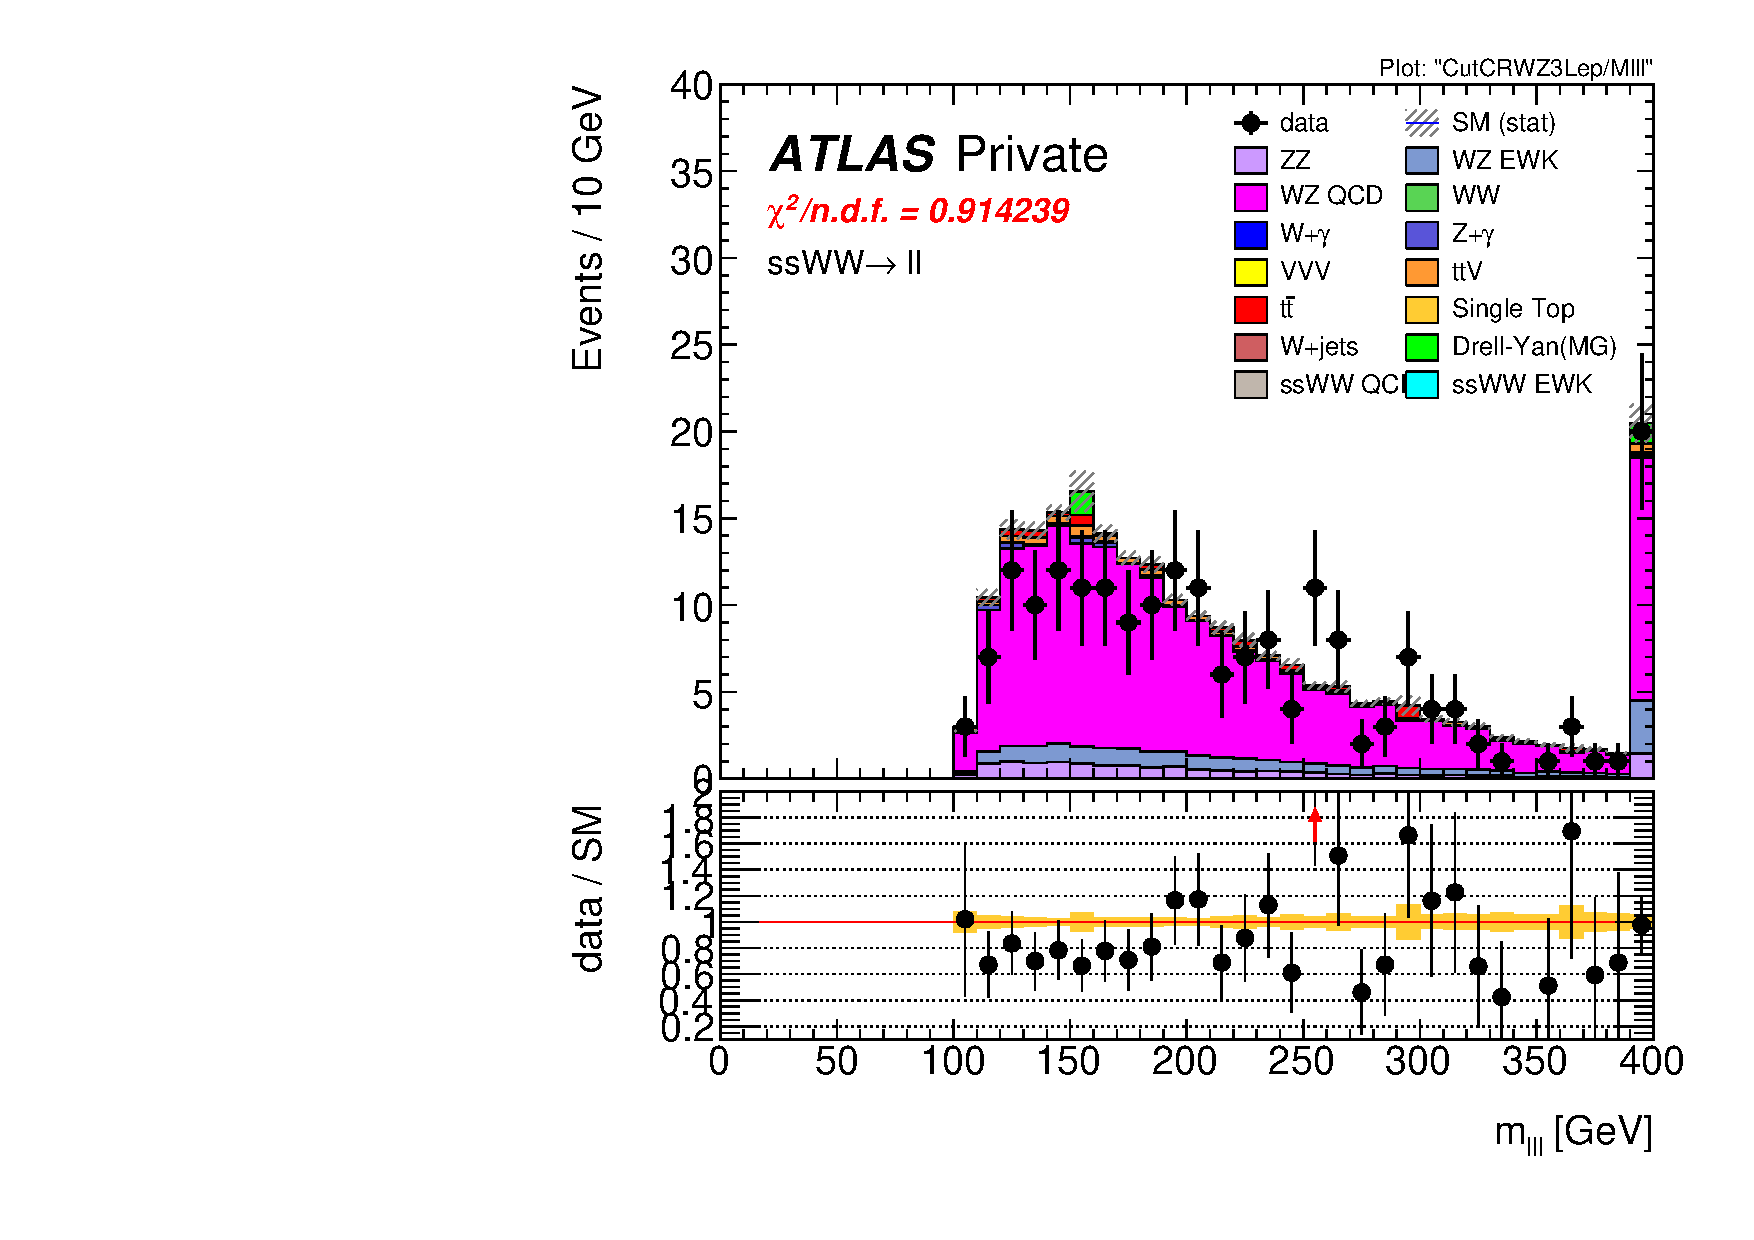
\includegraphics[width=.48\textwidth]{figs/ssww_13tev/backgrounds/wz/ll-CutCRWZ3Lep-Mlll-lin}
  \caption{Trilepton invariant mass $m_{lll}$ distribution in the $WZ$ control region before normalization.  All lepton channels are combined.}
  \label{fig:ssww13tev_wzcr_lep0}
\end{figure}

\subsection{Estimation of the $V\gamma$ background}\label{ssww13tev:wgamma}
Events from $V\gamma$ processes can pass selection if the photon converts into an $e^{+}e^{-}$ pair and one of the electrons passes the selection criteria.
The background is estimated from MC simulations which are then scaled by a normalization factor calculated from a control region enriched in $Z(\mu^{+}\mu^{-})\gamma$ events.
This control region selects two opposite-sign muons and an additional electron that is assumed to come from the photon conversion.
The full event selection is detailed in Table~\ref{tab:ssww13tev_vgamma_cr}.

\begin{table}[htbp]
  \centering
  \begin{tabular}{c}
    $V\gamma$ control region \\
    \hline\hline
    Exactly two muons with $\pt > 27\gev$ and $\pt > 20\gev$ \\
    Exactly one additional electron with $\pt > 15\gev$ \\
    Remove overlap between $Z$+jets and $Z\gamma$ \\
    Di-muon + photon invariant mass $75 < M_{\mu\mu\gamma} < 100\gev$ \\
    $\met < 30\gev$ \\
    \hline
  \end{tabular}
  \caption{Selection criteria for the $V\gamma$ control region.}
  \label{tab:ssww13tev_vgamma_cr}
\end{table}

The $Z\gamma$ MC samples available do not cover the full range of $\pt^\gamma$ and $\deltar(\gamma,l)$; thus, additional Drell-Yan samples ($Z$+jets) are used to fill out the phase space.
Overlap between the two samples are removed based to avoid double counting.
Events with final state photons at truth level are checked to ensure that the photon did not originate from a hadronic decay.
Cuts on $\pt^\gamma > 10\gev$ and $\deltar(\gamma,l) > 0.1$ are then applied at generator level, and $Z\gamma$ events that fail and $Z$+jets events that pass this additional selection are removed.

The normalization factor is calculated directly from the event yields in the $V\gamma$ control region rather than in the signal fit, as is done for the $WZ$ background.
The event yields are listed in Table~\ref{tab:ssww13tev_vgamma_numbers}, and the normalization factor is determined to be $1.77$.
No MC events from $Z\gamma$ processes survive the full event selection; thus, the scaling is only applied to the $W\gamma$ background in the signal region.
A systematic uncertainty of 44\% is assigned to the background based off of the uncertainties in the calculation of the normalization factor.

\begin{table}[htbp]
  \centering
  \begin{tabular}{l r}
    \multicolumn{2}{c}{Event yields in the $V\gamma$ control region} \\
    \hline\hline
    $Z\gamma$ & $24.6\pm 3.3$ \\
    $Z$+jets  &  $3.0\pm 1.5$ \\
    diboson + triboson & $6.7\pm 0.3$ \\
    top       &  $1.5\pm 0.5$ \\
    \hline
    Total prediction & $35.8\pm 3.7$ \\
    Data             & $57 \pm 7.6$ \\
    %\hline
    %Data - prediction & $21.2\pm 8.4$ \\
    \hline
  \end{tabular}
  \caption{Event yields in the $V\gamma$ control region.  The $V\gamma$ scale factor of 1.77 is calculated by scaling up the $Z\gamma$ and $Z$+jets backgrounds to account for the difference between the data and predicted total background.}
  \label{tab:ssww13tev_vgamma_numbers}
\end{table}

\subsection{Estimation of backgrounds from charge misidentification}\label{ssww13tev:charge_misid}
If an electron's charge is mis-reconstructed, it can lead to a real, opposite-sign lepton pair passing the same-sign requirement in the event selection.
There are two primary reasons this can occur:
\begin{enumerate}
\item An electron emits a photon via bremsstrahlung which then converts into an electron-positron pair, and the conversion track with the wrong electric charge is matched to the original electron.
This is the dominant process leading to charge flip, and it is highly dependent on the electron $\eta$ due to the different amount of detector material the electron passes through.
\item The curvature of the electron's track is mismeasured, resulting in the wrong charge being assigned.
This process is dependent on the momentum of the electron, as its track becomes more straight as the momentum of the electron increases.
\end{enumerate}

In order to estimate this background, the rate at which an electron's charge is misidentified is calculated from $Z\rightarrow e^{+}e^{-}$ MC simulation.
It is known that the MC does not perfectly model the material effects leading to charge flip; as a result, scale factors are applied to the MC in order for it to to better reflect the real performance.
These scale factors are obtained from the ratio of charge mis-ID rates in data and uncorrected MC in~\cite{2018.ssww-13tev-atlas-support} following the method outlined in~\cite{2017.charge-flip-support}.
Once the scale factors are applied, the charge misidentification rate $\varepsilon$ can be extracted by comparing the electron's reconstructed charge with the charge of its truth particle:
\begin{equation}
  \varepsilon(\eta,\pt) = \frac{N_{\textrm{wrong\ charge}}}{N_{\textrm{prompt\ electrons}}}
\end{equation}
The charge mis-ID rate is calculated in bins of electron $|\eta|$ and $\pt$ and varies from below $0.1\%$ in the central region of the detector up to $8\%$ in the forward regions for high $\pt$ (above $90\gev$) electrons.
A two-dimensional plot of $\varepsilon$ can be found in Figure~\ref{fig:charge_flip_rates}.

\begin{figure}
  \centering
  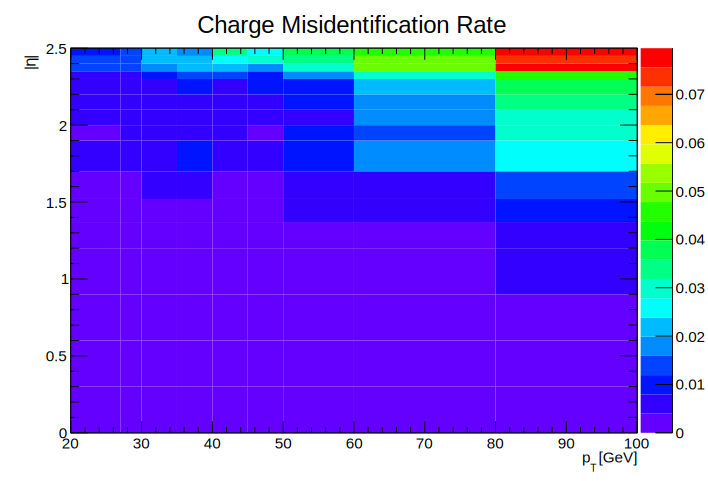
\includegraphics[width=.7\textwidth]{figs/ssww_13tev/backgrounds/charge_flip/charge_flip_2d}
  \caption{Charge misidentification rates for electrons as a function of $|\eta|$ and $\pt$.  Rates are calculated from $Z\rightarrow e^{+}e^{-}$ MC after applying sacle factors to approximate the charge mis-ID rates in data.}
  \label{fig:charge_flip_rates}
\end{figure}

%The size of the charge mis-ID background in a given region (signal or control region) is estimated from events that pass the region's default event selection but with an opposite-sign lepton pair.
Given the charge flip rate $\varepsilon(\eta,\pt)$, the rate at which an electron has its charge correctly reconstructed is $(1-\varepsilon)$.
Thus there are three possible combinations of charge identification, assuming a two-electron event:
\begin{enumerate}
\item Both electrons are reconstructed correctly: $(1-\varepsilon)^2$
\item Both electrons are mis-reconstructed: $\varepsilon^2$
\item Only one electron is mis-reconstructed: $2\varepsilon(1-\varepsilon)$
\end{enumerate}

In order to estimate the size of the background from charge misidentification, opposite-sign events are selected using the default event selection for a given signal or control region with the same-sign requirement inverted.
These events are then weighted by the probability for one of the electrons to be reconstructed with the wrong charge:
\begin{equation}
\omega = \frac{\varepsilon_1(1-\varepsilon_2)+\varepsilon_2(1-\varepsilon_1)}{(1-\varepsilon_1)(1-\varepsilon_2)+\varepsilon_1\varepsilon_2}
\label{ssww13tev:ch_flip_weight}
\end{equation}
%\begin{equation}
%\omega = \frac{\varepsilon_1(1-\varepsilon_2)+\varepsilon_2(1-\varepsilon_1)}{1-(\varepsilon_1+\varepsilon_2)+2\varepsilon_1\varepsilon_2}
%\label{ssww13tev:ch_flip_weight2}
%\end{equation}
where the subscripts 1 and 2 refer to the leading and subleading electrons, respectively, and $\varepsilon_i$ is a function of the $\eta$ and $\pt$ of the $i^{\textrm{th}}$ electron.
In the case of an event with only one electron and one muon, Equation~\ref{ssww13tev:ch_flip_weight} simplifies:
\begin{equation}
\omega = \frac{\varepsilon}{1-\varepsilon}
\end{equation}
This method assumes that there is little contamination from fake electrons in the opposite-sign sample, and this has been verified with MC simulation.

Additionally, charge-flipped electrons tend to be reconstructed with lower energy when compared to electrons with the correct charge.
This is due to energy loss from the material interactions that can cause the charge to be misidentified.
A correction factor is calculated from MC simulations, comparing the $\pt$ of the truth electron to its reconstructed counterpart:
\begin{equation}
\alpha = \frac{\Big(\frac{\pt^{\textrm{reco}}}{\pt^{\textrm{truth}}}-1\Big)_{\textrm{correct charge}}}{\Big(\frac{\pt^{\textrm{reco}}}{\pt^{\textrm{truth}}}-1\Big)_{\textrm{wrong charge}}}
\label{ssww13tev:ch_flip_alpha}
\end{equation}
The correction is then applied to the $\pt$ of the charge-flipped electron via
\begin{equation}
\pt = \pt^0/(1+\alpha)+dE
\label{ssww13tev:ch_flip_energy_corr}
\end{equation}
where $\pt^0$ is the uncorrected $\pt$ of the electron and $dE$ is a gaussian smearing factor centered at zero with a width related to the energy resolution.
Since which electron is misreconstructed is never determined in this method, in the case of a two-electron event, the energy correction is applied randomly to one of the two electrons based on the probabilities for them to be charge-flipped.
This also determines the overall sign of the event; the charge of the electron that does not recieve the correction is taken to be the charge for both.

Systematic uncertainties on the charge mis-ID rates are calculated by generating two additional sets of rates with the uncertainties on the scale factors varied up and down.
The size of the estimated charge flip background without the energy correction applied is also taken as a systematic uncertainty.
These systematic uncertainties are estimated to be approximately $\pm 15\%$.

\subsubsection{Validation of the charge misidentification estimate}\label{ssww13tev:ssincl_vr}
%The performance of the charge misidentification estimation is tested in $e^{\pm}e^{\pm}$ events with a di-electron invariant mass that lies within $15\gev$ of the $Z$ boson mass.
%Disagreements between data and background at high $\pt$ and $\eta$ have been found to be due to backgrounds from misidentified leptons, which are not included due to unreliable modeling in this particular region.

The performance of the charge misidentification estimation is tested in the same-sign inclusive validation region (VR), defined in Table~\ref{tab:ssww13tev_ssincl_vr_def}.
For $ee$ events, the mass of the dilepton pair is required to lie within $15\gev$ of the $Z$ boson mass to increase the purity of the charge flip background.
$t\bar{t}$ production, which can contribute to both the charge mis-ID and fake lepton backgrounds, is suppressed by the $b$-jet veto.
The di-electron invariant mass is shown in Figure~\ref{fig:ssww13tev_ssincl_mll}, and distributions of the leading and subleading electron $\pt$ in the $ee$-channel are shown in Figure~\ref{fig:ssww13tev_ssincl_ptlep} with the $Z$ mass cut inverted.
Agreement between data and prediction is seen within the total statistical and systematic uncertainties in the VR.

\begin{table}[htbp]
  \centering
  \begin{tabular}{c}
    Same-sign inclusive VR \\
    \hline\hline
    Exactly 2 same-sign signal leptons\\
    $\pt > 27\gev$ for both leptons \\
    $m_{ll} > 20\gev$\\
    $|m_{ee} - m_Z| > 15\gev$ ($\ee$-channel only) \\
    $N_{b\textrm{-jet}} = 0$\\
    \hline
  \end{tabular}
  \caption{Selection criteria for the same-sign inclusive validation region.}
  \label{tab:ssww13tev_ssincl_vr_def}
\end{table}

\begin{figure}
  \centering
  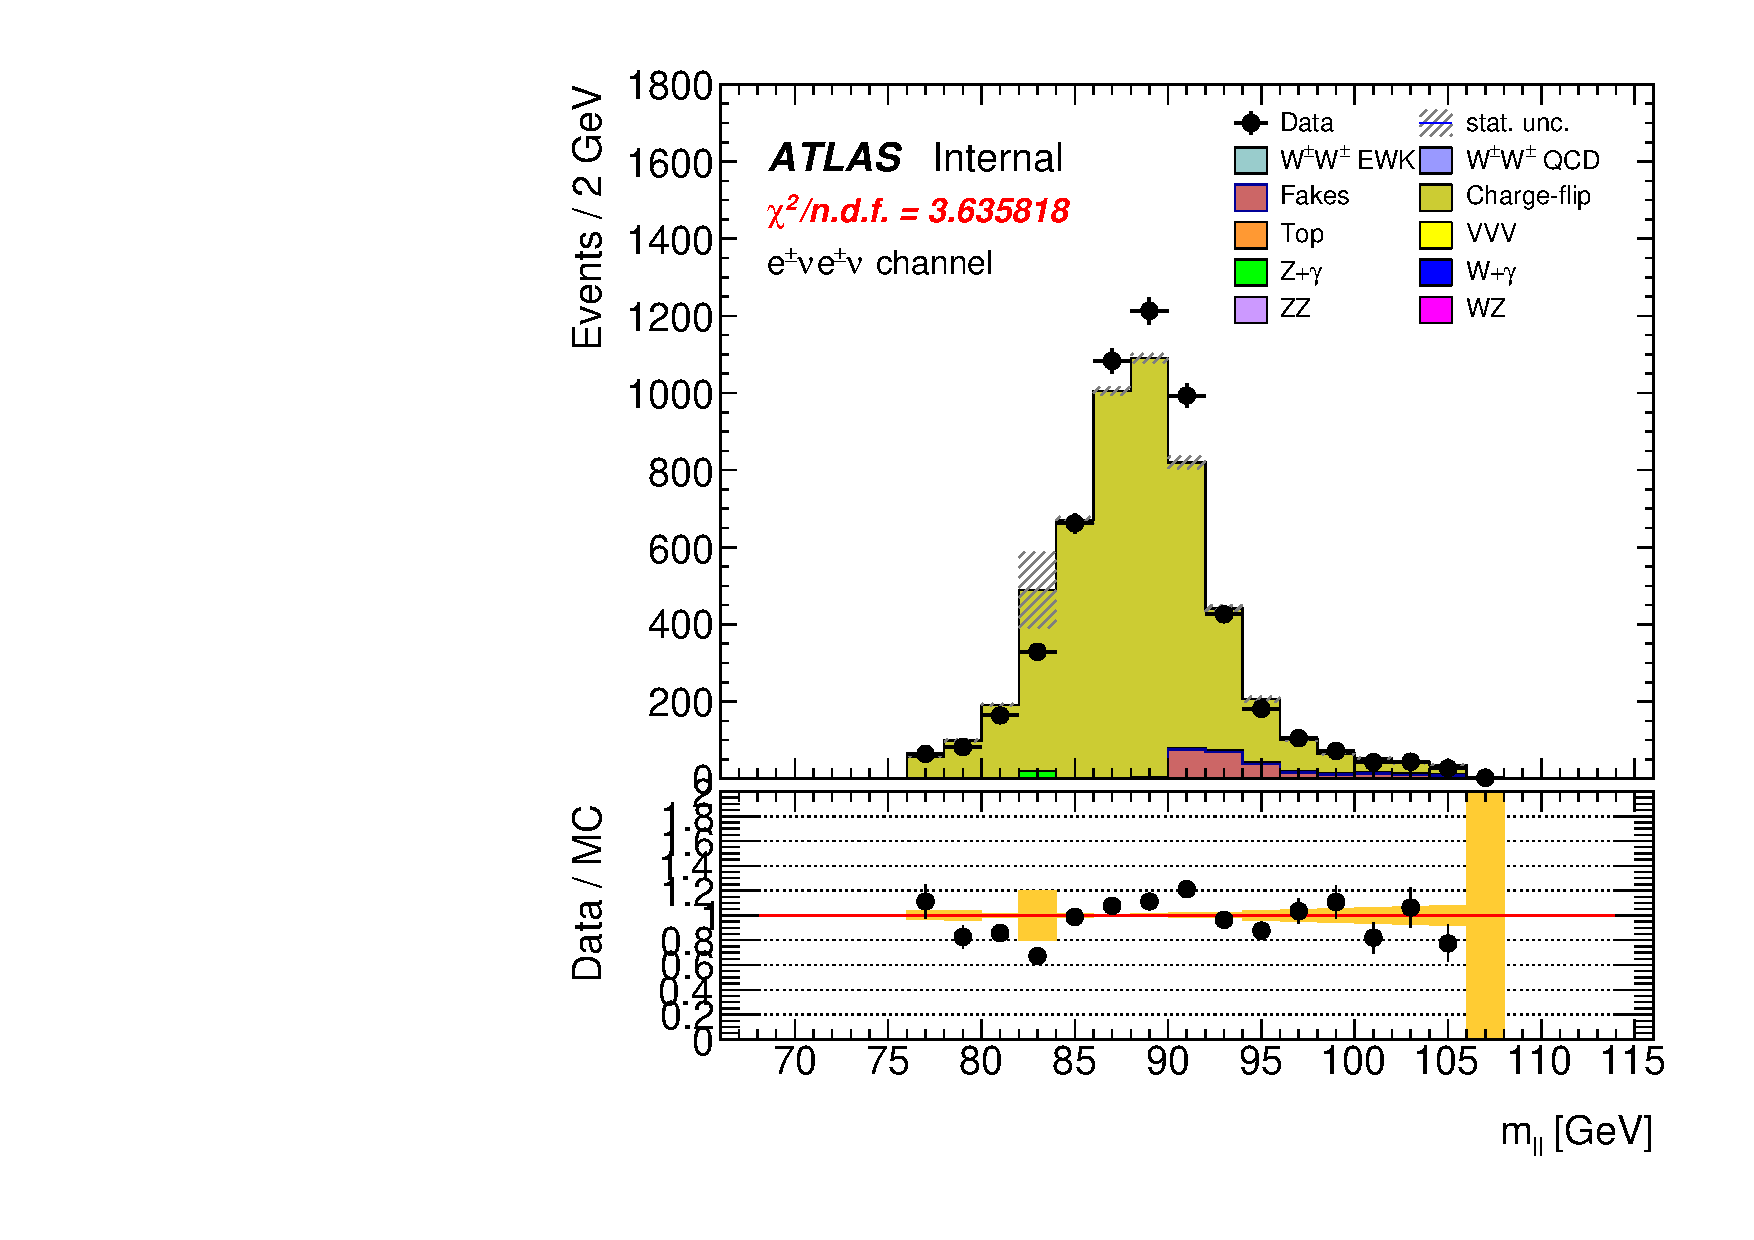
\includegraphics[width=.48\textwidth]{figs/ssww_13tev/backgrounds/charge_flip/ee-CutCRInclusiveSSZ-Mll_Zpeak-lin}
  \caption{Dilepton invariant mass distribution $m_{ll}$ for the $ee$ channel in the same-sign inclusive VR.}
  \label{fig:ssww13tev_ssincl_mll}
\end{figure}

\begin{figure}
  \centering
  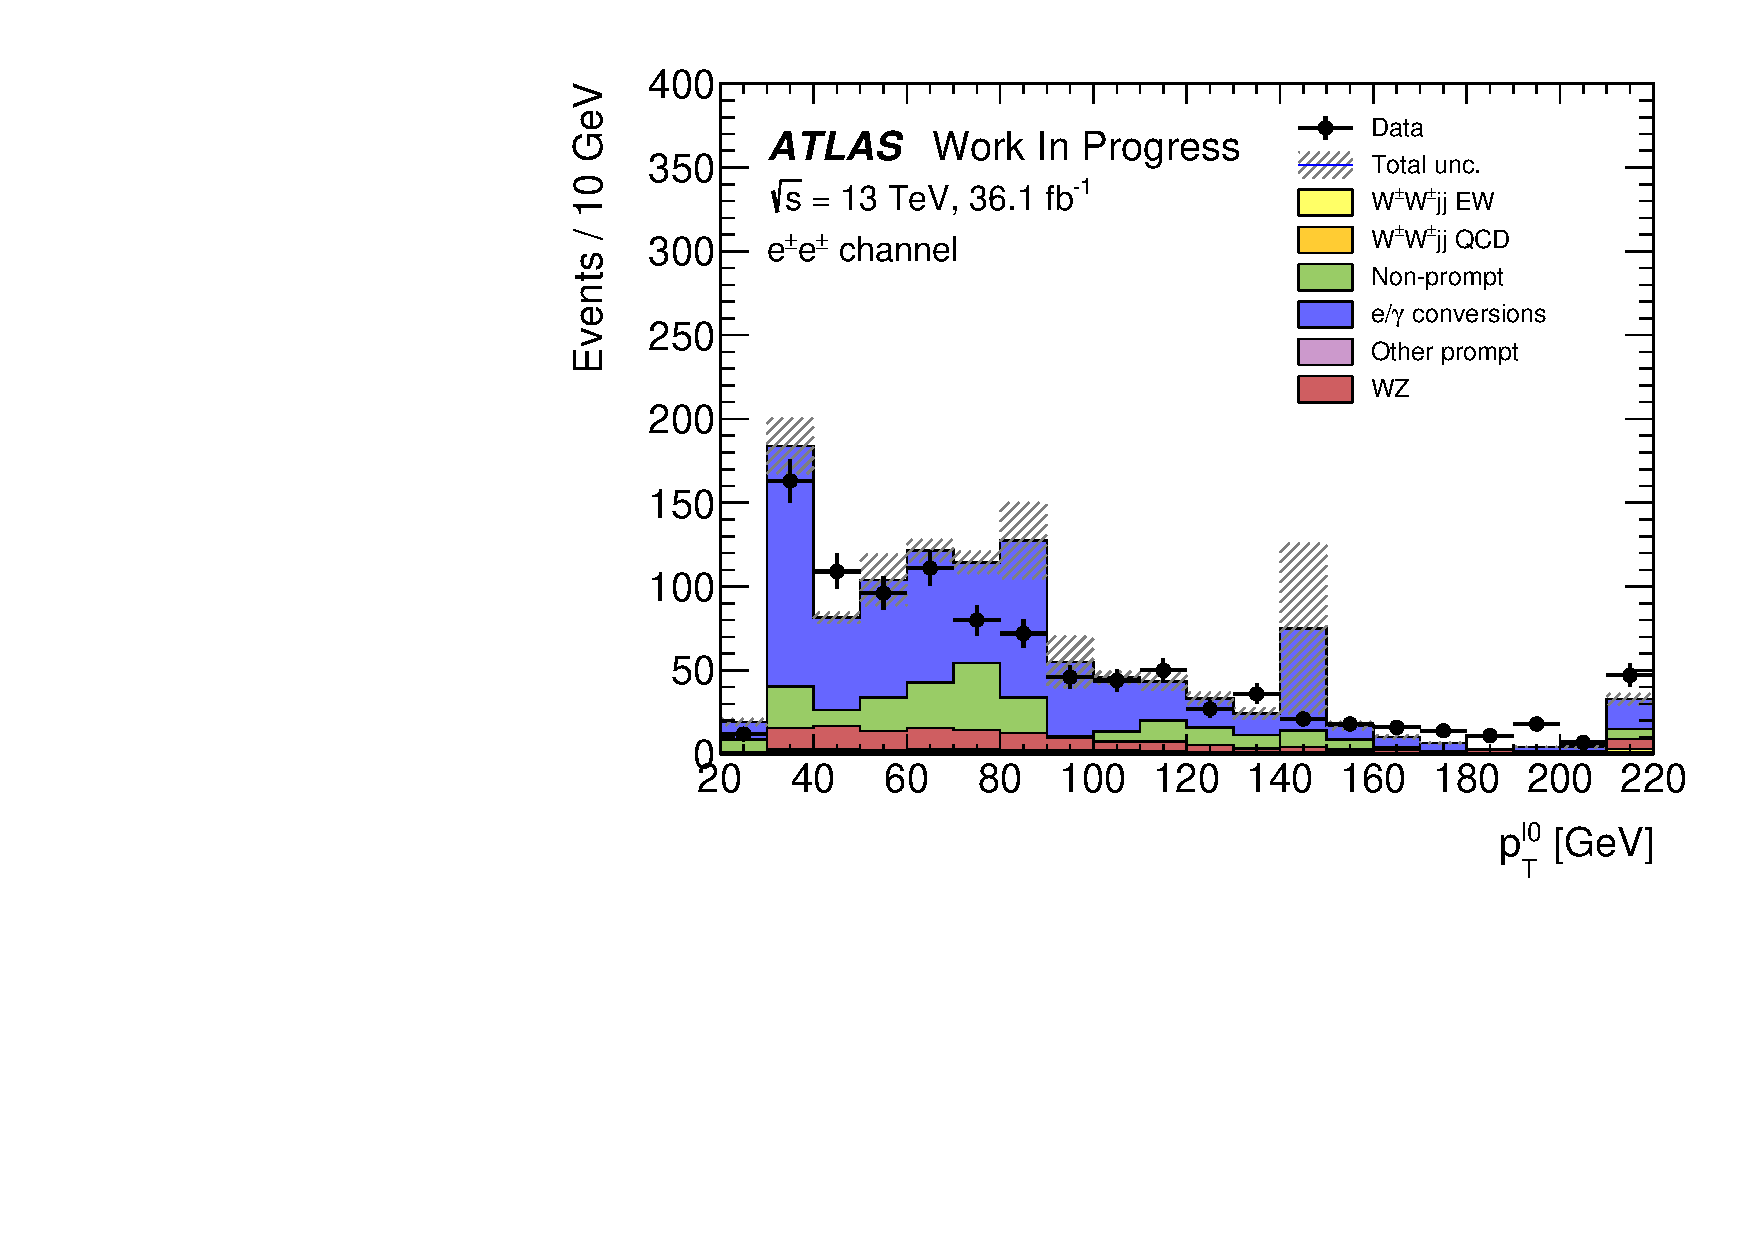
\includegraphics[width=.48\textwidth]{figs/ssww_13tev/backgrounds/charge_flip/ee-CutCRInclusiveSSZVeto-l0_pt-lin.pdf}
  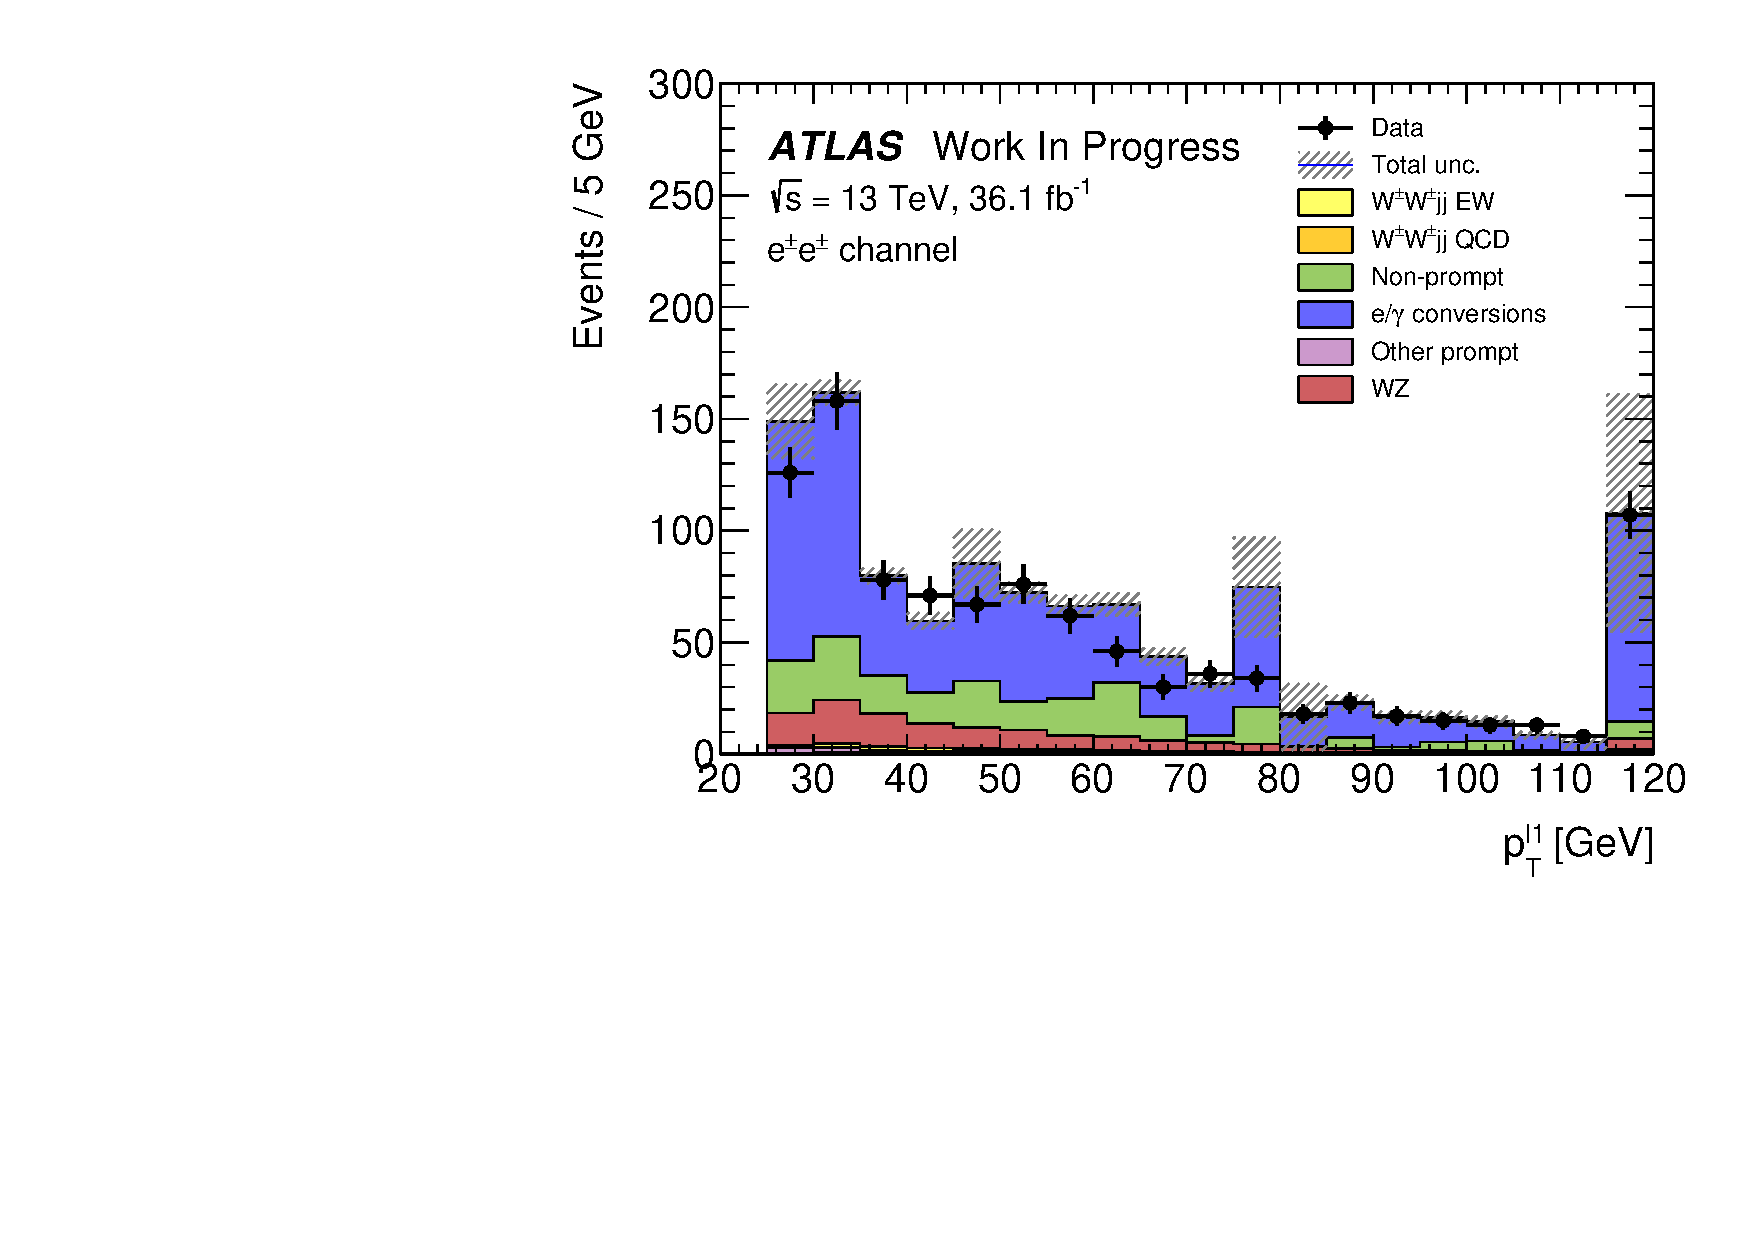
\includegraphics[width=.48\textwidth]{figs/ssww_13tev/backgrounds/charge_flip/ee-CutCRInclusiveSSZVeto-l1_pt-lin.pdf}
  \caption{$\pt$ distributions for the leading (left) and subleading (right) electron for the $ee$ channel in the same-sign inclusive VR.  In these plots, the cut requiring $m_{ee}$ to fall within the $Z$ mass window has been inverted in order to test the modelling away from the $Z$ peak.}
  \label{fig:ssww13tev_ssincl_ptlep}
\end{figure}

\subsection{Estimation of non-prompt backgrounds with the fake factor method}\label{ssww13tev:fake_factor}
fake factor method


\subsection{Reduction of $WZ$ background using custom overlap removal}\label{ssww13tev:custom_or}
The dominant source of prompt background in this analysis comes from $WZ$ events where both bosons decay leptonically.
Traditionally, the background is dealt with by imposing a veto on any event with a third lepton passing some loose identification criteria (the so-called \emph{trilepton veto}).
In the case of this analysis, if one or more leptons (in addition to the two signal leptons) passed the preselection criteria, the event would be rejected.
However, $WZ$ events can still enter the signal region if one of the leptons fails the veto selection or falls outside of the detector's acceptance.

In order to understand the sources of $WZ$ events that are not removed by the trilepton veto, a study was performed on truth-level leptons\footnote{Truth particles are the particles produced directly by the MC generator before being passed through the full detector simulation, at which point they are considered \emph{reconstruction-level} (or \emph{reco-level}) particles.} on \ssww and $WZ$ MC samples.
Events with three truth leptons were selected, and each was matched to its reconstruction-level partner by finding the closest $\deltar(\textrm{truth},\textrm{reco})$ and $\Delta p_{\textrm{T},\textrm{truth},\textrm{reco}}$ match.
For events surviving the trilepton veto, the two signal leptons were removed, and the remaining leptons represent real leptons that failed to be selected for the veto.
Between 40-50\% of these leptons fell outside of the eta acceptance of the analysis (see Figure~\ref{fig:ssww13tev_wzveto_truthlepeta}) and were unrecoverable.
The second largest source of leptons failing the preselection was the overlap removal (OR). \TODO{Make sure to define overlap removal in the event selection section!}
The standard OF procedure appeared to be too aggressive in removing leptons in favor of jets, causing many three lepton events to ``lose'' their third lepton and pass the trilepton veto.

\begin{figure}[htbp]
  \centering
  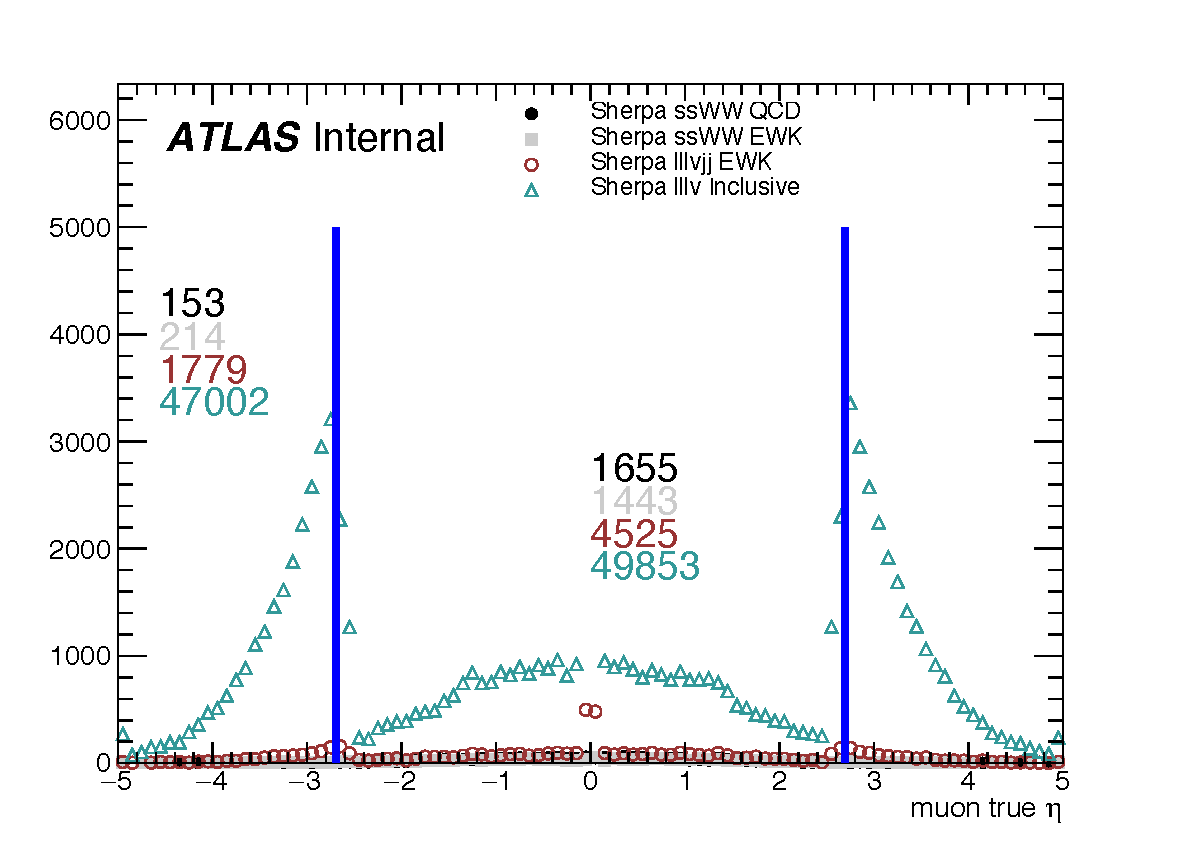
\includegraphics[width=.48\textwidth]{figs/ssww_13tev/custom_or/ExtraMuonEta_counted}
  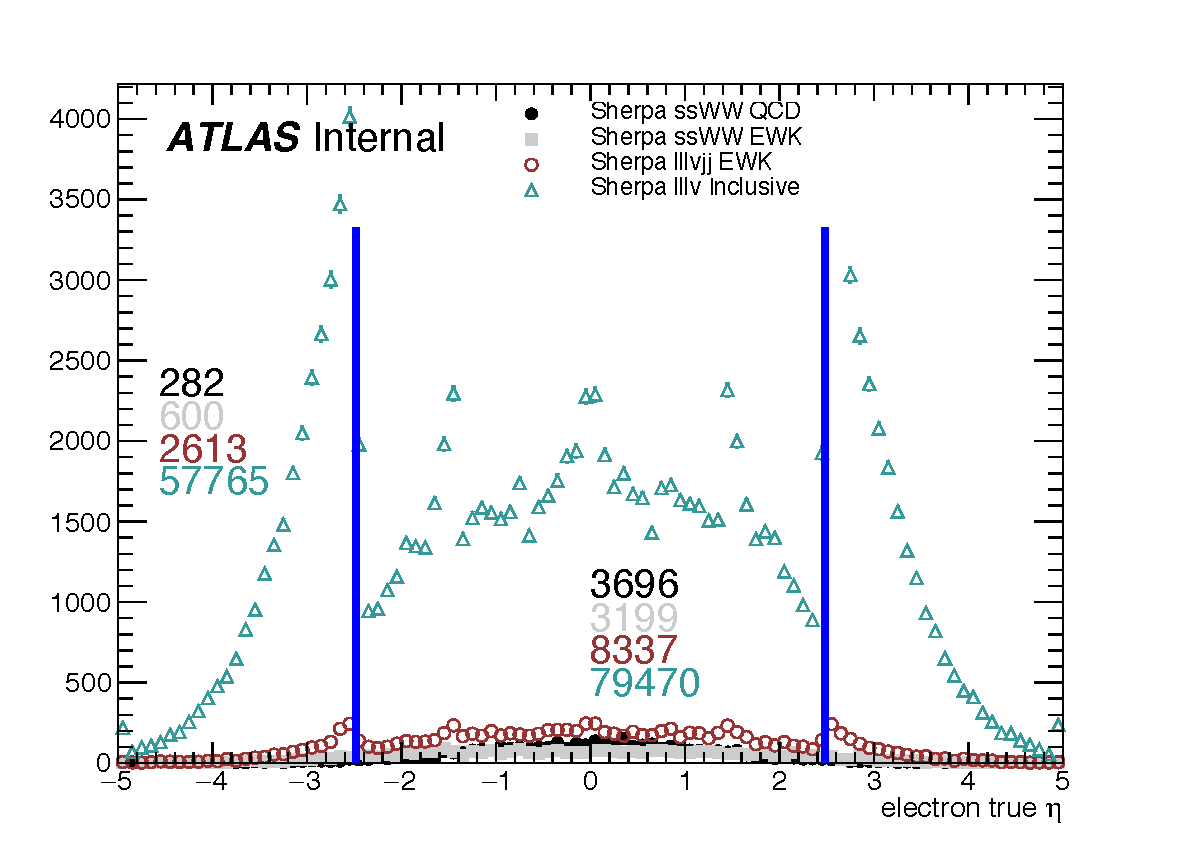
\includegraphics[width=.48\textwidth]{figs/ssww_13tev/custom_or/ExtraElecEta_counted}
  \caption{Pseudorapidity ($\eta$) distributions of truth muons (top) and electrons (bottom) for Sherpa \ssww and $WZ$ MC samples.  The blue vertical lines represent the allowed $\eta$ range for each lepton flavor.  The numbers correspond to the number of raw MC events that fall within and outside of the allowed $\eta$ range for each MC sample.}
  \label{fig:ssww13tev_wzveto_truthlepeta}
\end{figure}

Two quantities were chosen to construct a ``custom'' OR that would 

\begin{figure}[htbp]
  \centering
  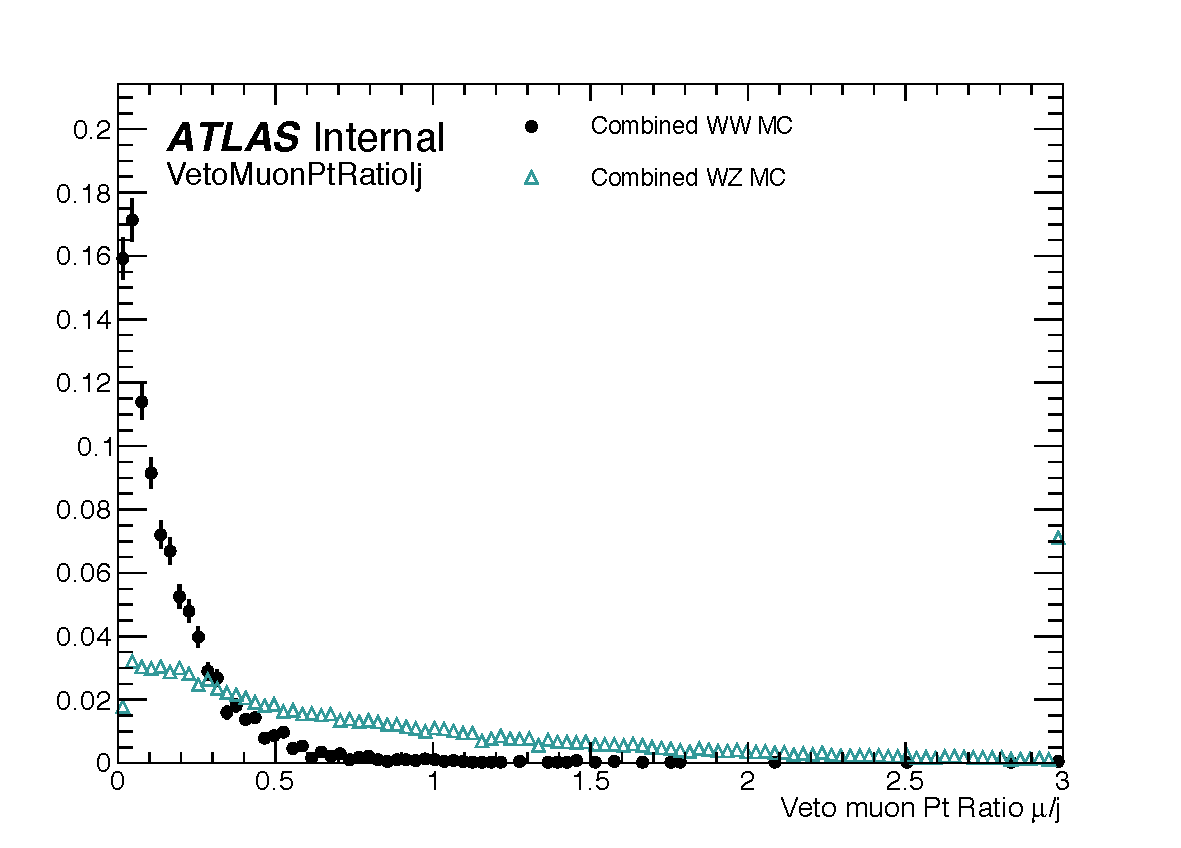
\includegraphics[width=.48\textwidth]{figs/ssww_13tev/custom_or/VetoMuonPtRatiolj}
  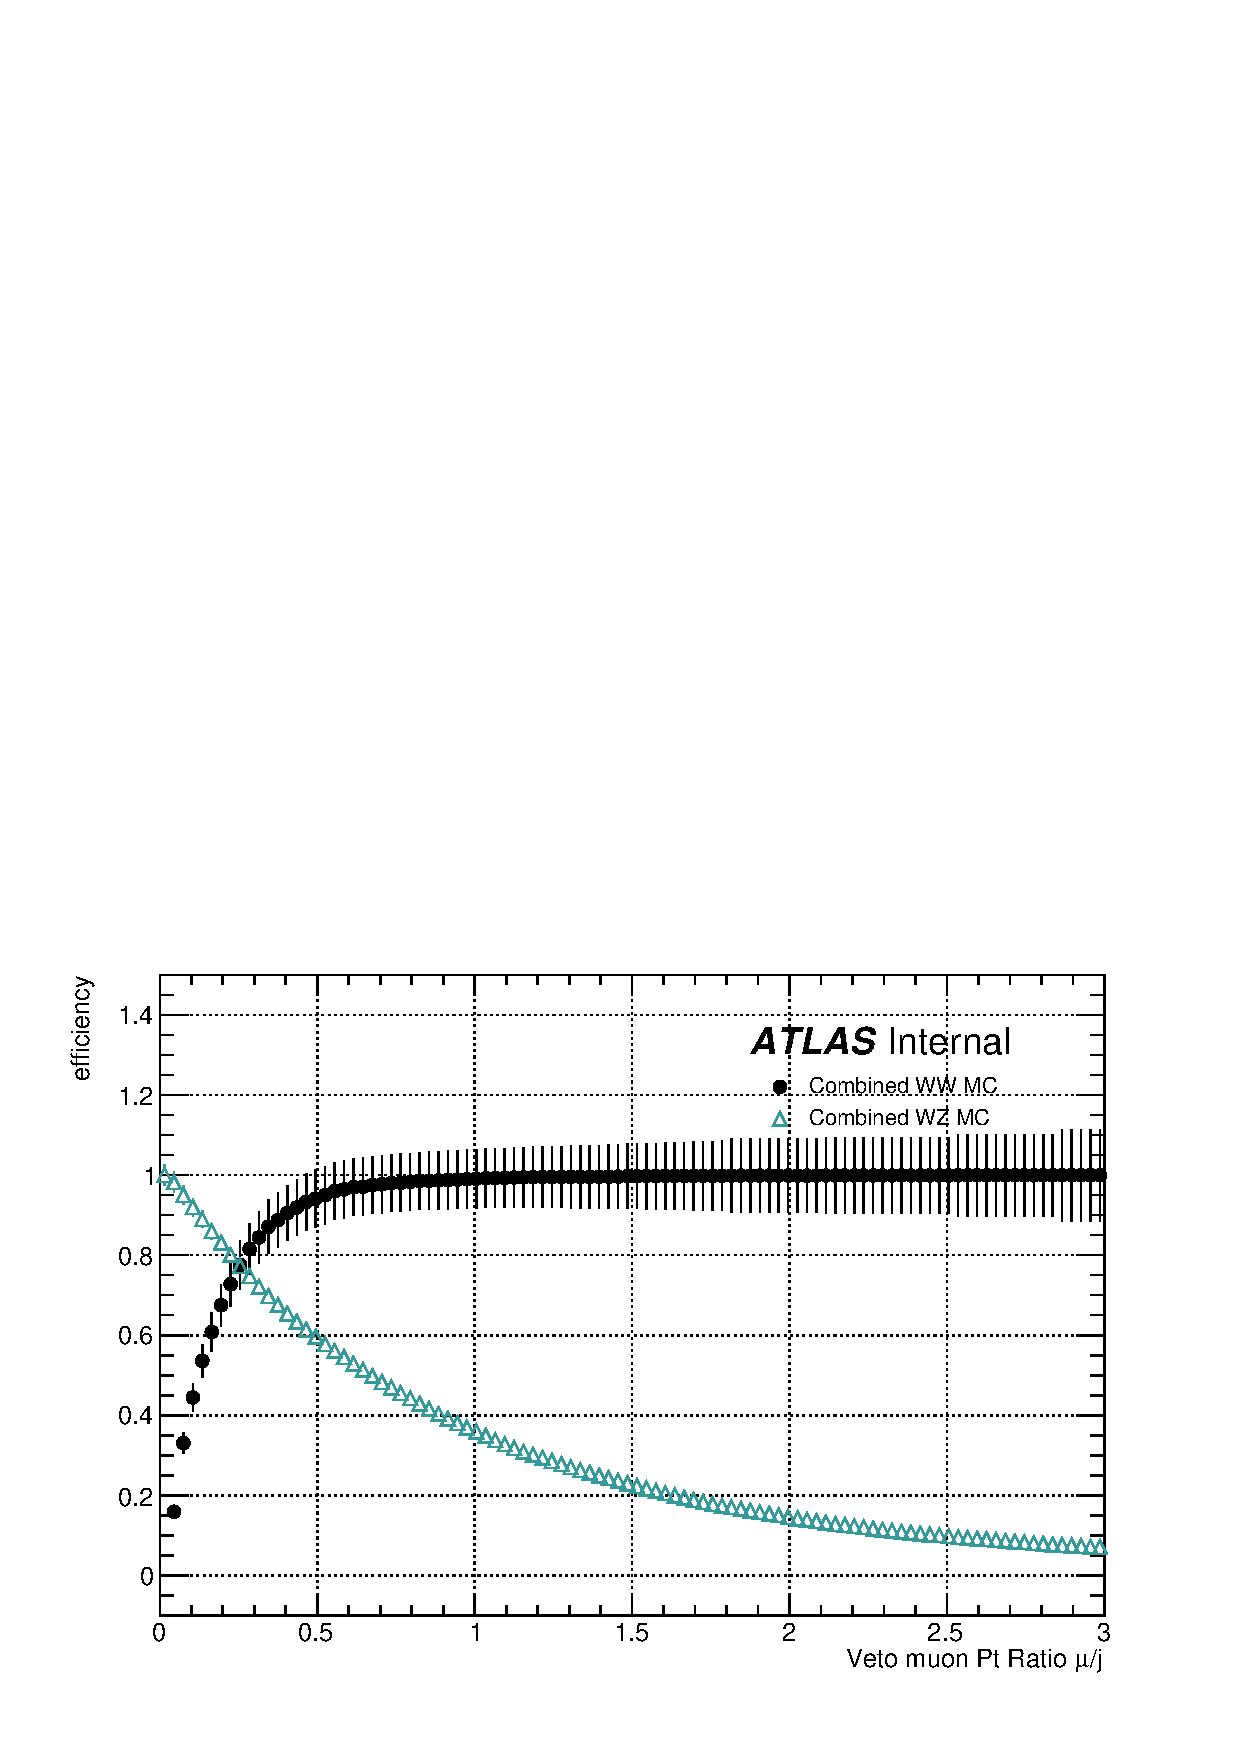
\includegraphics[width=.48\textwidth]{figs/ssww_13tev/custom_or/ROC_VetoMuonPtRatiolj}\\
  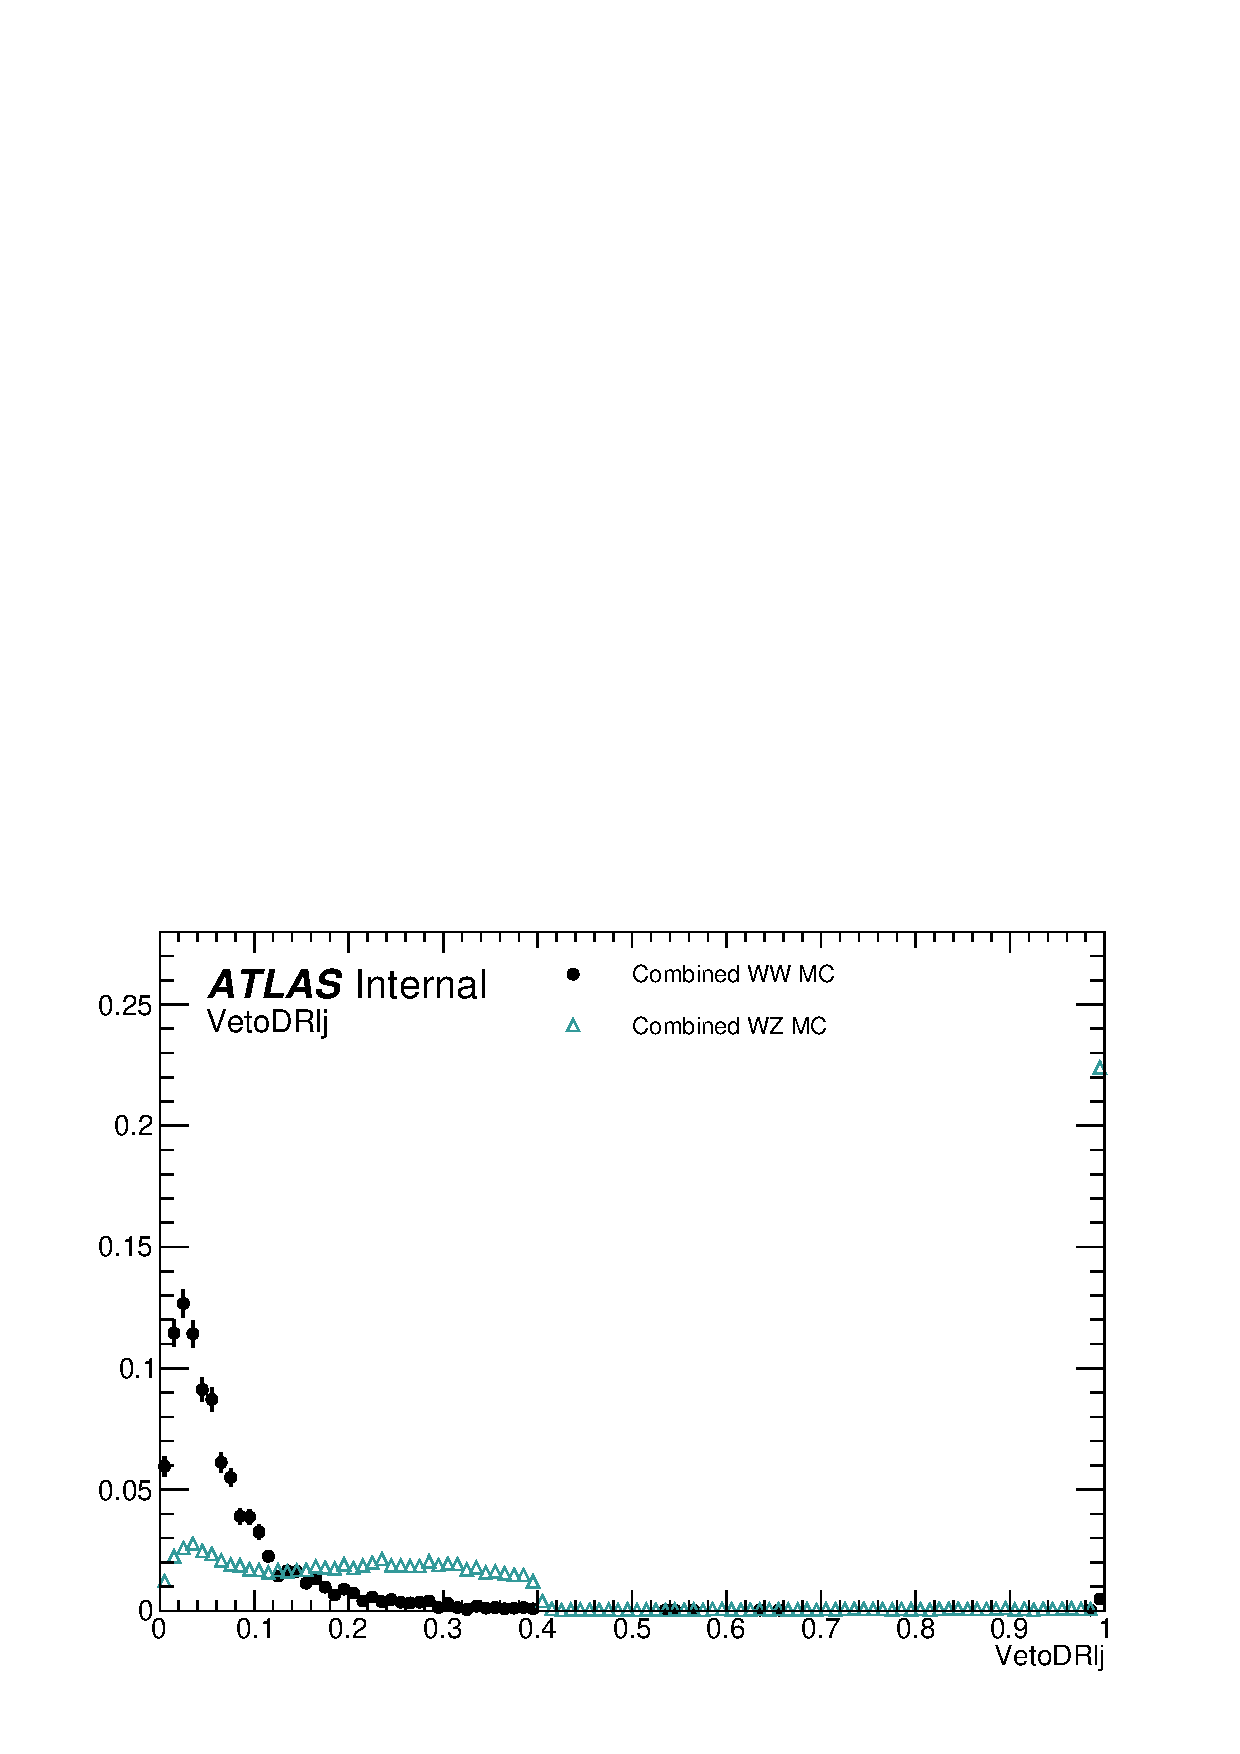
\includegraphics[width=.48\textwidth]{figs/ssww_13tev/custom_or/veto_muon_VetoDRlj}
  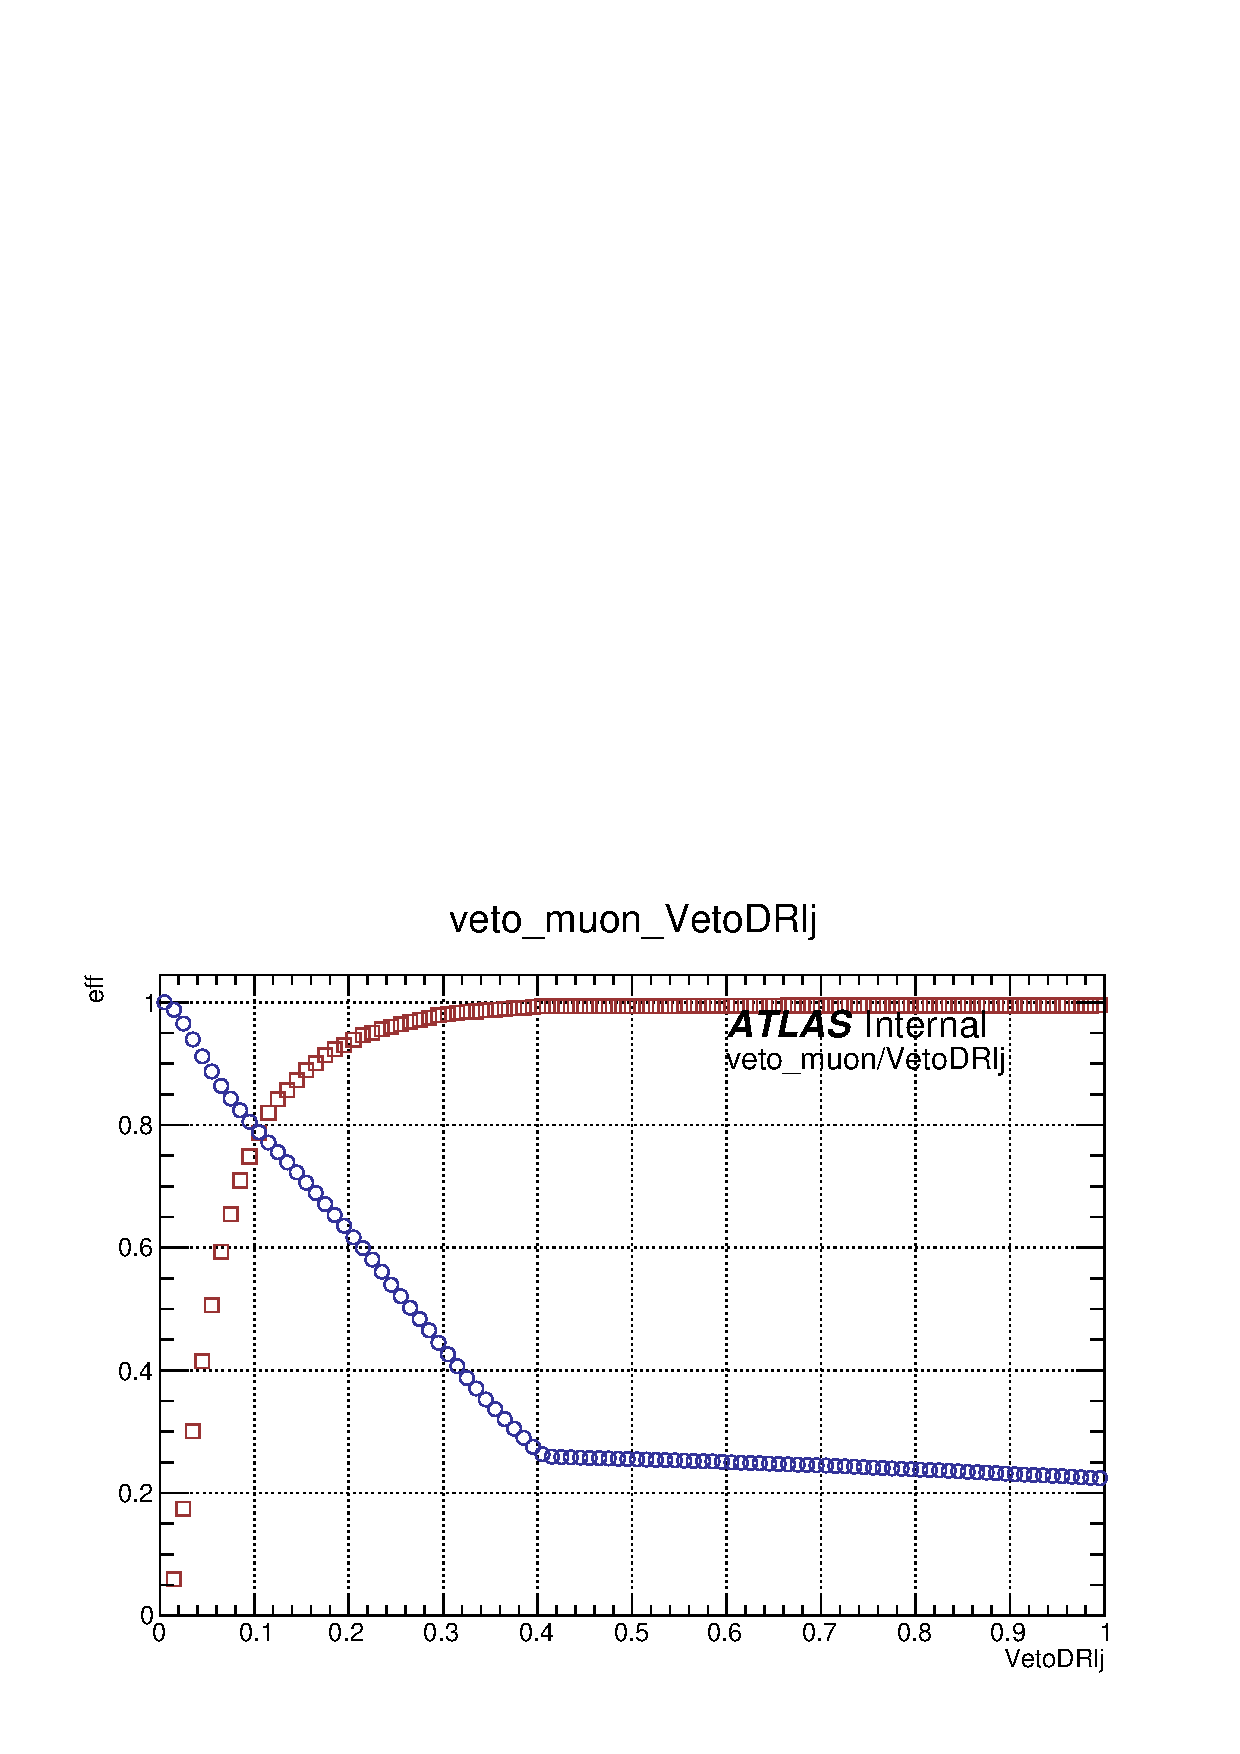
\includegraphics[width=.48\textwidth]{figs/ssww_13tev/custom_or/ROC_veto_muon_VetoDRlj}\\
  \caption{Stuff}
  \label{fig:ssww13tev_customor_muon}
\end{figure}

\begin{figure}[htbp]
  \centering
  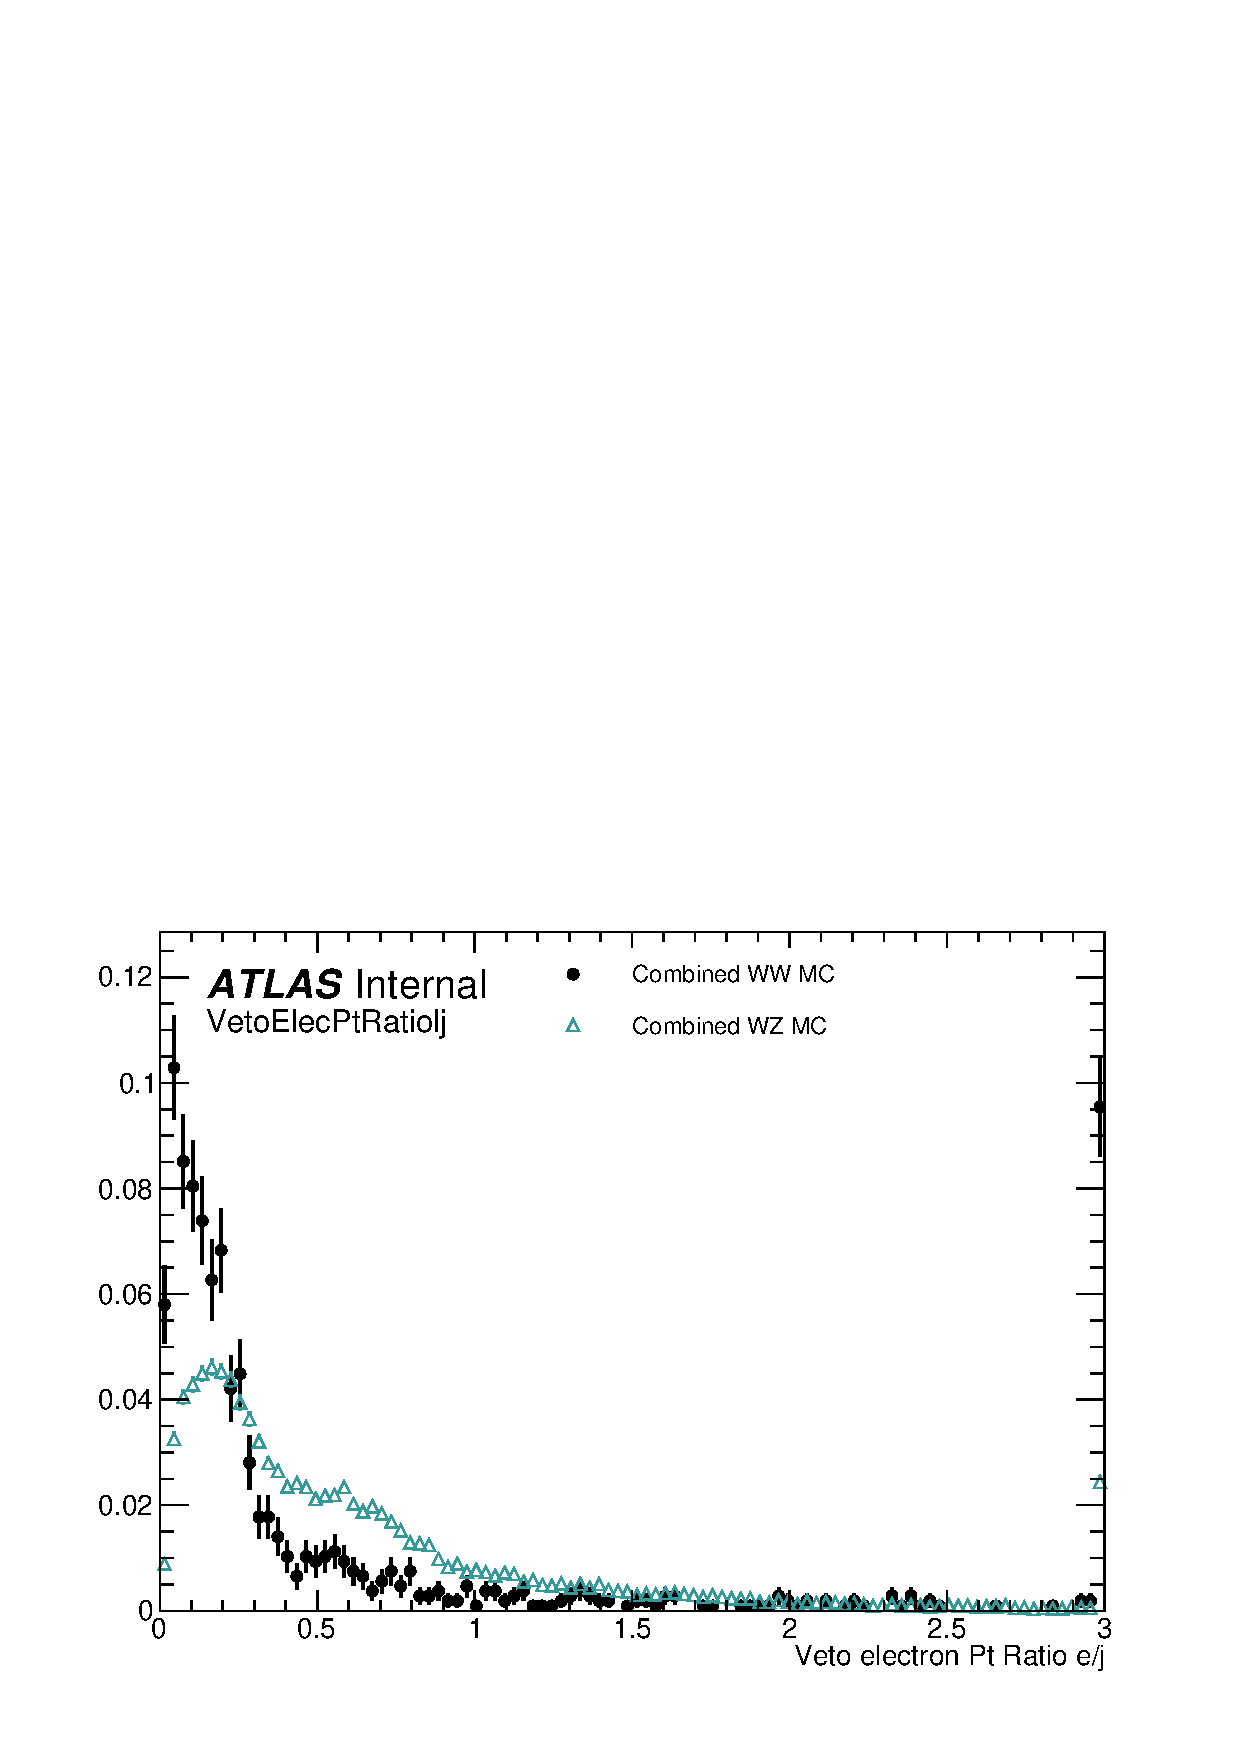
\includegraphics[width=.48\textwidth]{figs/ssww_13tev/custom_or/VetoElecPtRatiolj}
  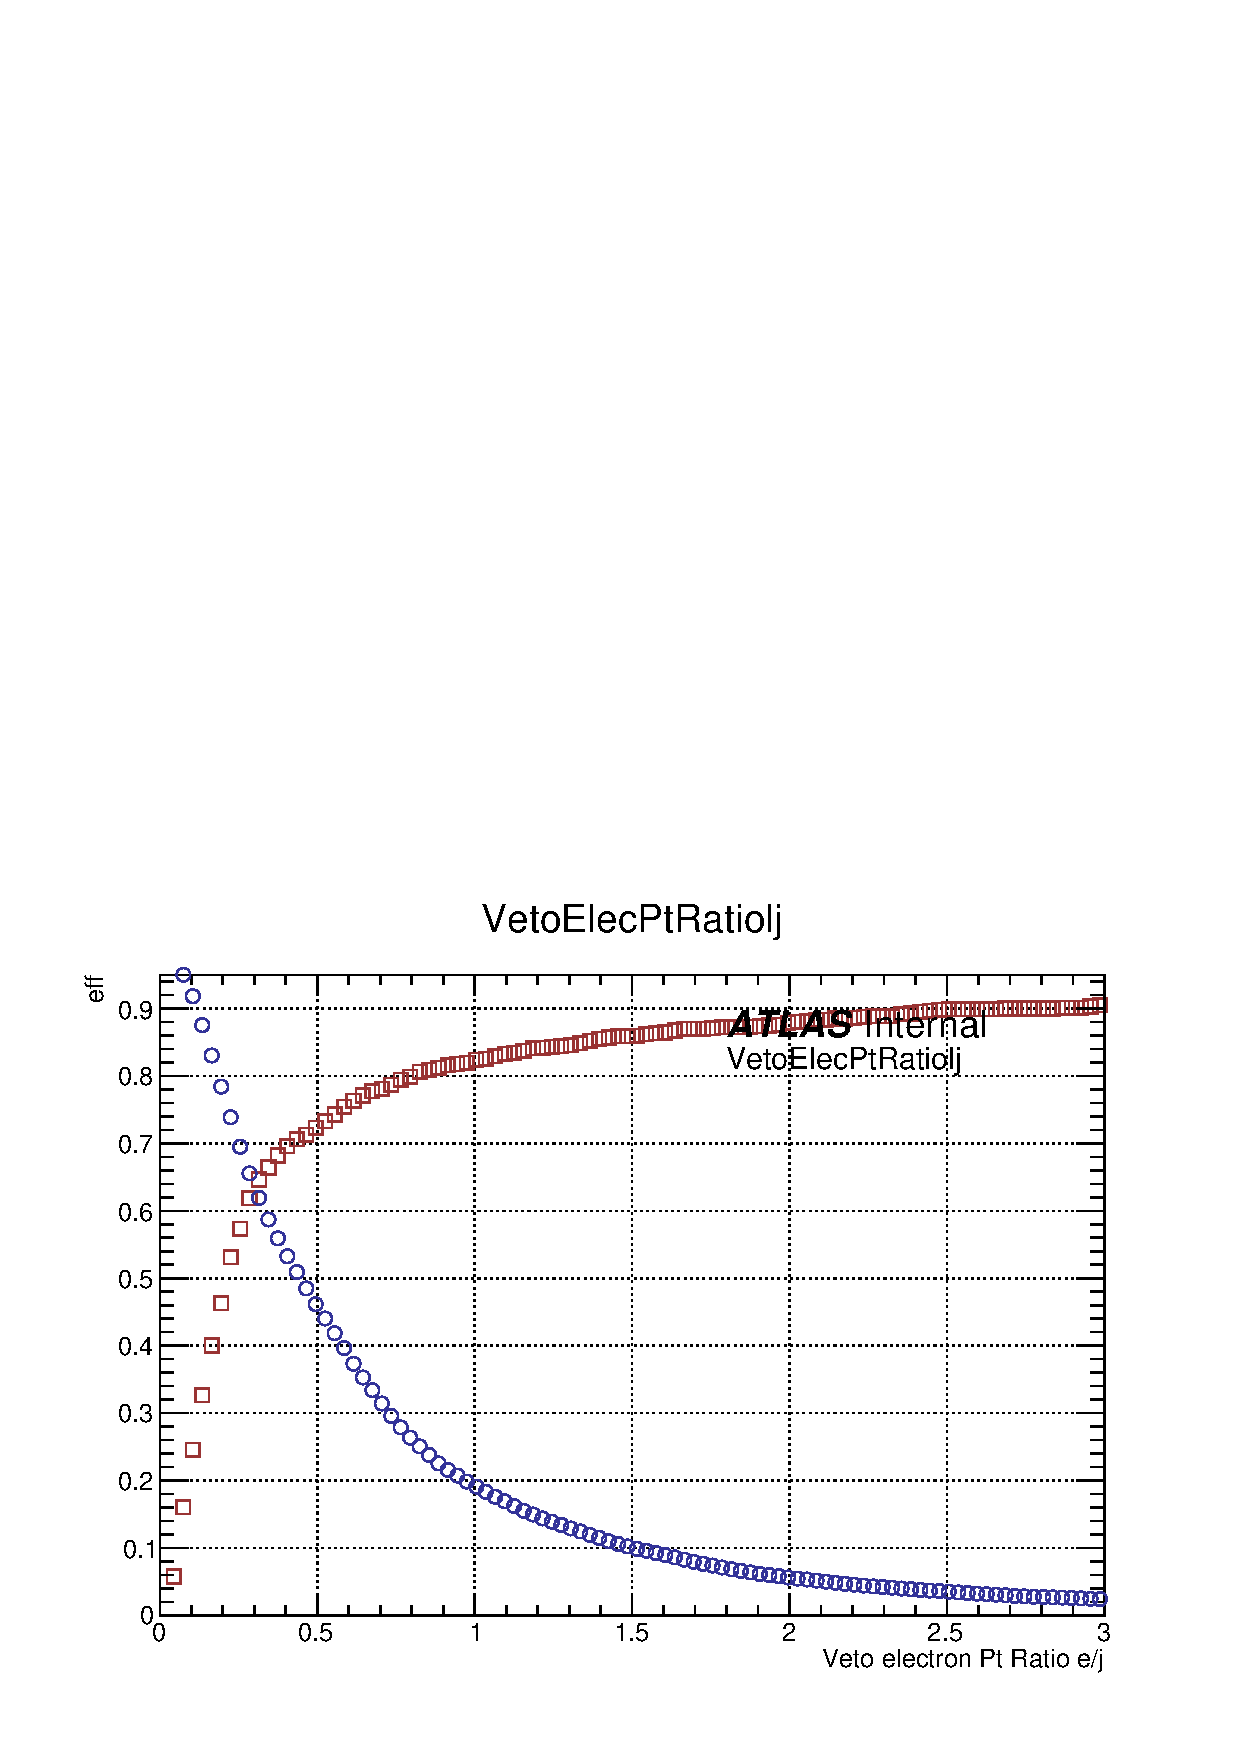
\includegraphics[width=.48\textwidth]{figs/ssww_13tev/custom_or/ROC_VetoElecPtRatiolj}
  \caption{Stuff}
  \label{fig:ssww13tev_customor_elec}
\end{figure}

\begin{figure}[htbp]
  \centering
  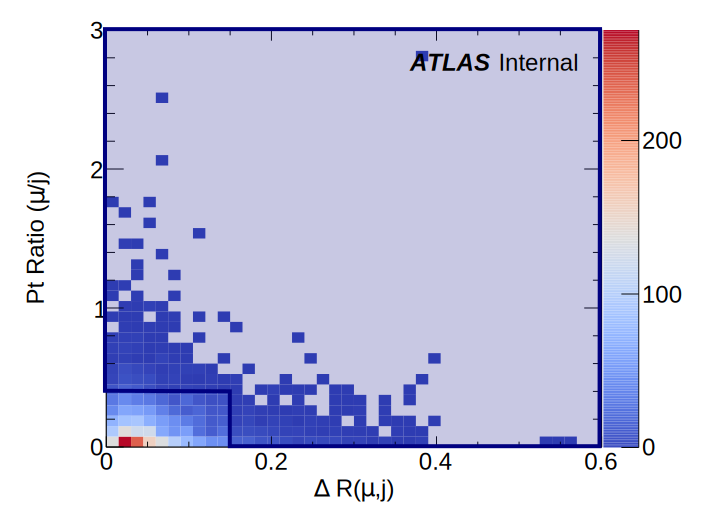
\includegraphics[width=.48\textwidth]{figs/ssww_13tev/custom_or/sig_Muon_DR_PtRatio_edited}
  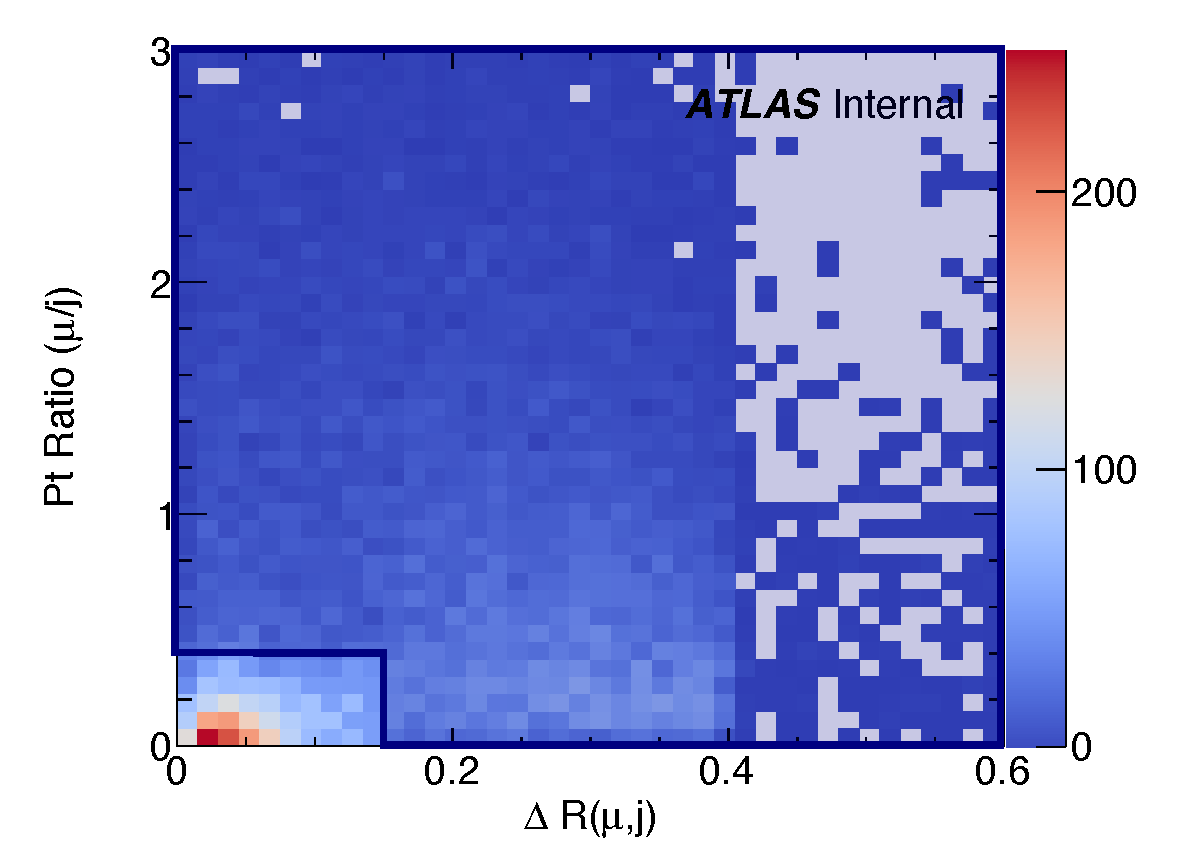
\includegraphics[width=.48\textwidth]{figs/ssww_13tev/custom_or/bkg_Muon_DR_PtRatio_edited}
  \caption{Stuff}
  \label{fig:ssww13tev_customor_muon_2d}
\end{figure}


